\section{Hojas de datos}
\label{sec:hojas-datos}

Las hojas de datos normalmente son archivos PDF.  En \LaTeX{} hay dos formas de insertar archivos PDF.  La más sencilla es utilizar la orden \texttt{includegraphics} que ya hemos visto en las figuras, pero solo se puede incrustar una página en cada llamada a \texttt{includegraphics}. 

Si el documento tiene varias páginas habría que insertar cada una de las páginas de interés con órdenes \texttt{includegraphics} independientes.  En el parámetro \texttt{page} podemos elegir la página a insertar.  Este método nos da el máximo control para poder poner pies de figura y el posicionamiento.  Sin embargo, cuando el documento tiene muchas páginas es un poco engorroso.  Para esos casos se puede utilizar la orden \texttt{includepdf} del paquete \emph{pdfpages}.

Para ilustrarlo veamos el mismo ejemplo, primero con \texttt{includepdf} y luego con \texttt{includegraphics}.

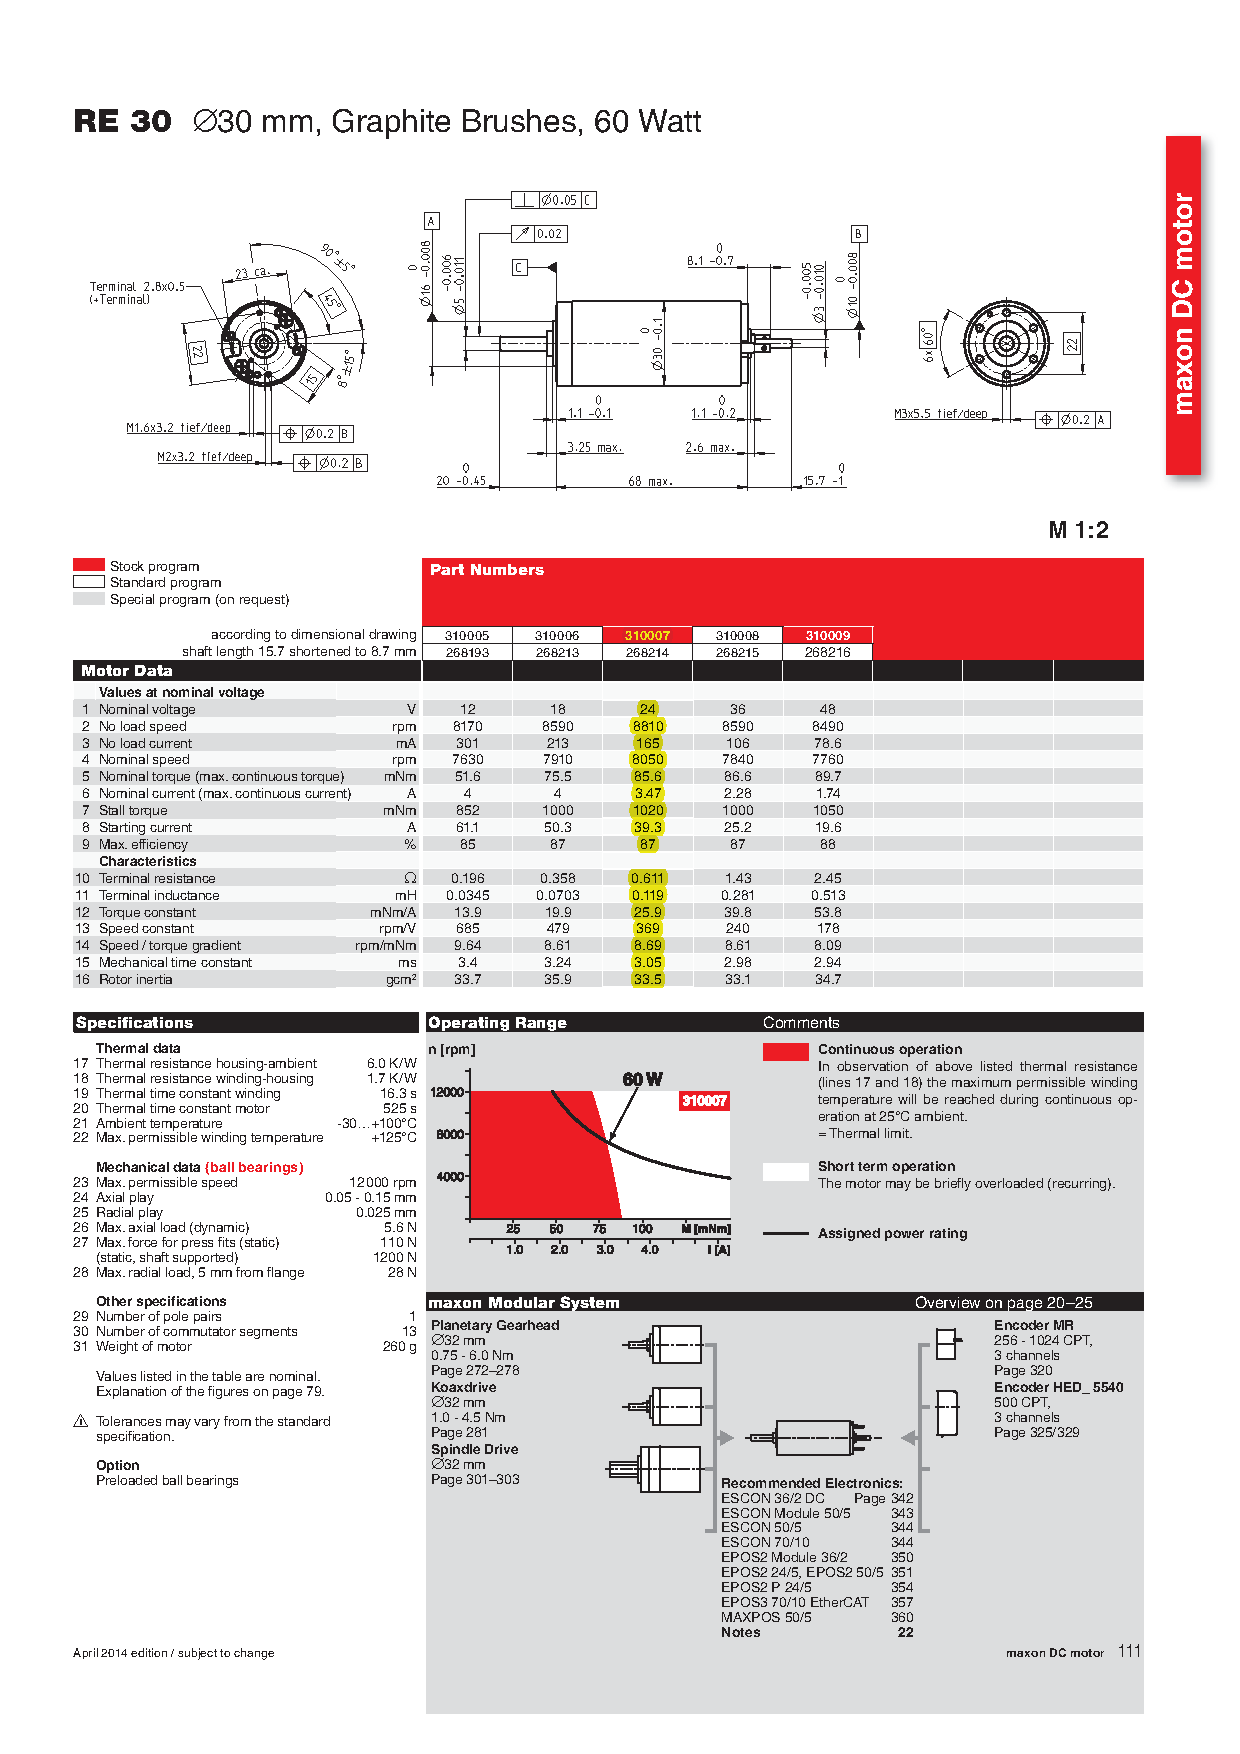
\includepdf[pages={1-},scale=0.8,pagecommand={}]{RE30.pdf}

La opción con \texttt{includegraphics} permite referirse a una página concreta y poner pies de figura.  Por ejemplo, en la figura~\ref{fig:hoja-datos} se muestra la hoja de especificaciones del motor empleado.

\begin{figure}[!ht]
\centering
\fbox{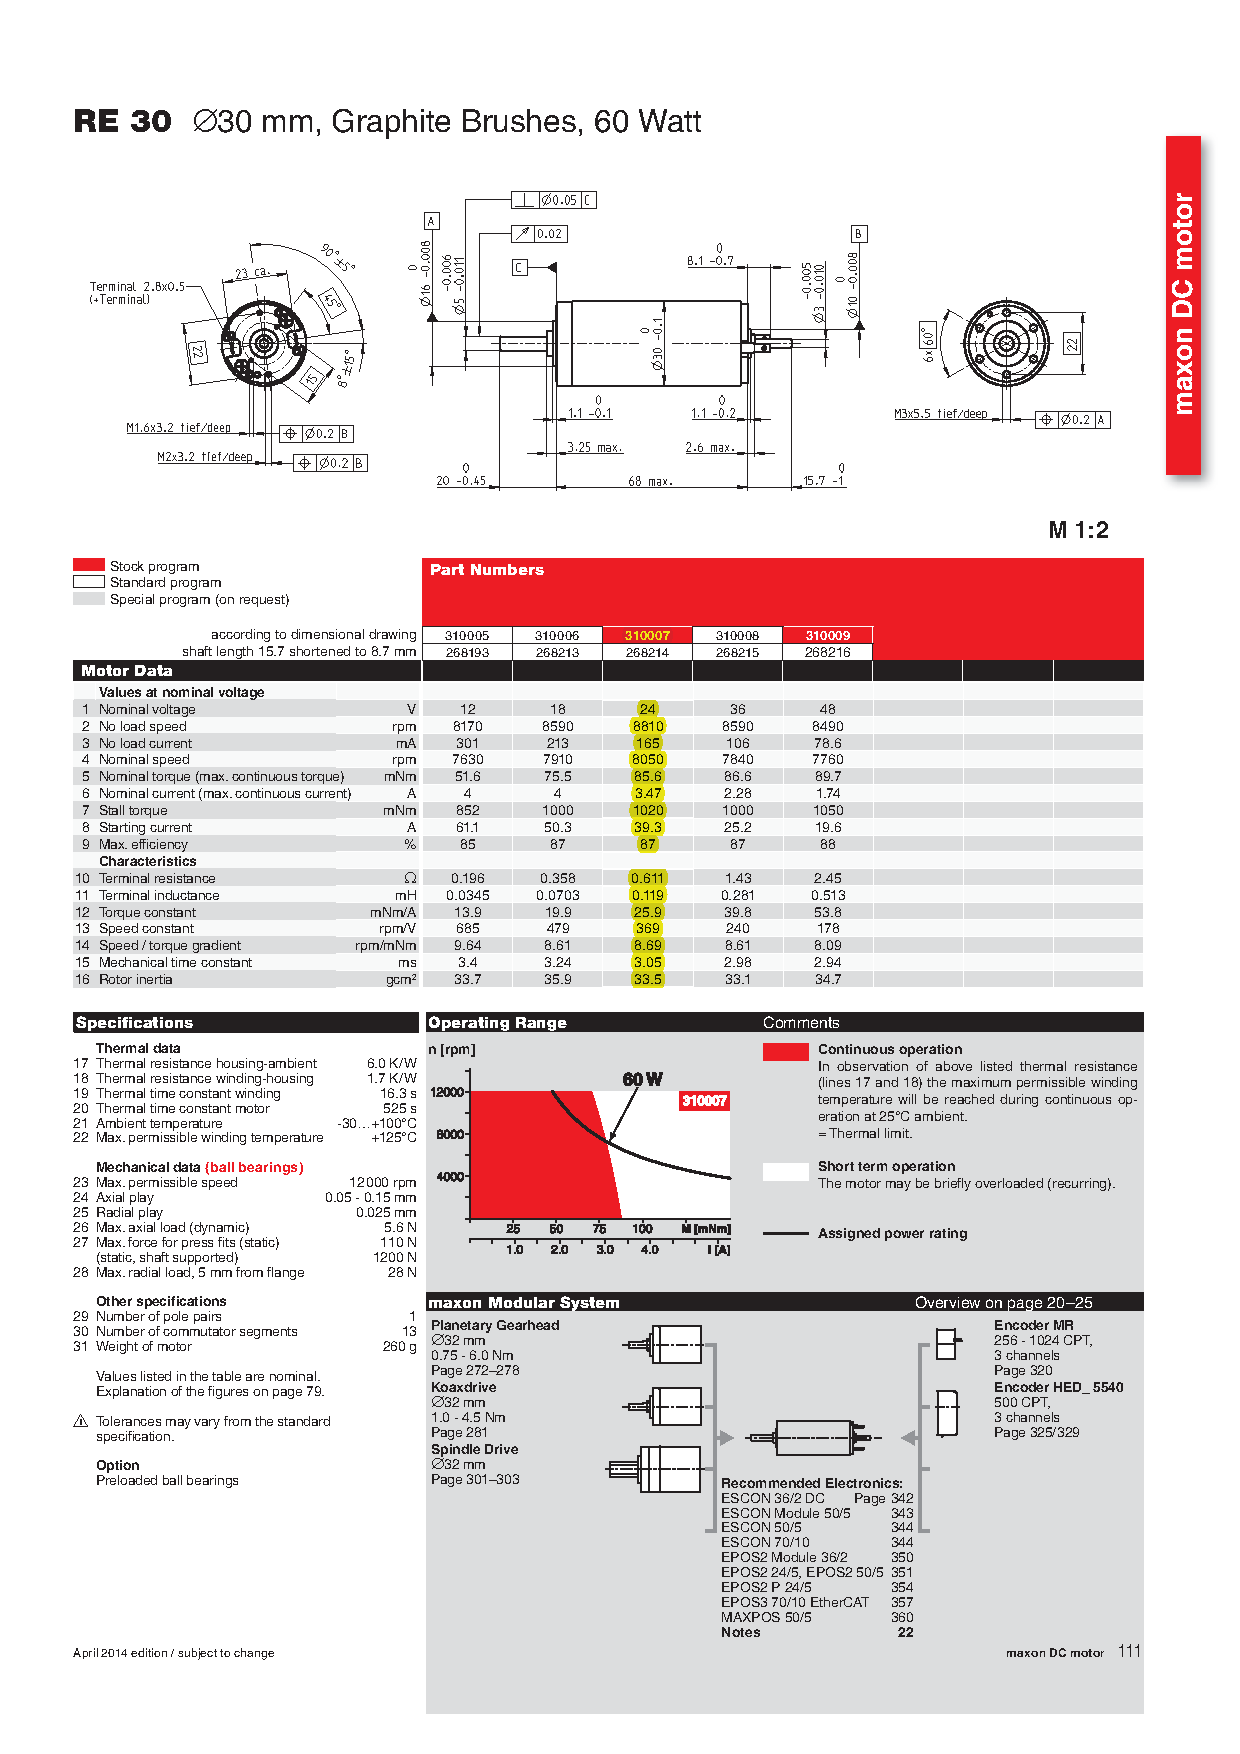
\includegraphics[page=1,width=.95\textwidth]{RE30.pdf}}
\caption{Figura ejemplo. Tomada de hoja de catálogo de \href{https://datasheets.globalspec.com/ds/17/MaxonPrecisionMotors/F1B48EDA-7358-46E6-964A-97E3BC5D921A}{motores DC con escobillas de grafito de Maxon} \copyright~2014 Maxon Motors. Reproducida con permiso.}
\label{fig:hoja-datos}
\end{figure}
